\documentclass[12pt]{article}

% set margins to something reasonable
\usepackage[left=1in, right=1in, top=1in, bottom=1in]{geometry}

\usepackage{titling}
\usepackage{siunitx}
\usepackage{booktabs}
\usepackage{amssymb,amsmath}
% \usepackage{gensymb}
\usepackage{graphicx}
\usepackage{float}



\usepackage{caption}
\captionsetup[table]{labelsep=none}


\providecommand{\e}[1]{\ensuremath{\times 10^{#1}}}


% header
\title{Short Spacing Issues for Mapping Extended Emission: Milky Way Case Study \\ {\Large ngVLA Memo \#54}}
\author{Jordan A.~Turner, Peter Teuben, Daniel A.~Dale}
\date{\today}

% end of preamble

\begin{document}

\maketitle

\begin{abstract}
The​ ​ next​ ​ generation​ ​ Very​ ​ Large​ ​ Array​ ​ will​ ​ provide​ ​ unprecedented​ ​ resolution​ ​ and​ ​ sensitivity​ ​ at radio​ ​ frequencies​ ​ from​ ​1 to​ 115​ ​ GHz. Like any interferometric array, the ngVLA will not cover all possible baselines and thus it will be limited in its ability to recover the true flux for all observed spatial scales. We present a detailed study of simulations carried out by adding various short spacing antennae configurations (large single-dish and closely packed compact array) to the interferometric data. The simulated observations make use of the newly developed Quick Array Combinations (QAC) CASA add-on derived from the TP2VIS project. We find the best flux recovery of simulated Milky Way extended emission when combining the ngVLA \textit{Short Baseline Array} and \textit{Core} antennae with a \SI{45}{\meter} diameter or larger single dish. In addition to the flux recovery, we also find a large single-dish total power option is needed to recover structures at large spatial scales. 
\end{abstract}

\section*{Introduction}

The next generation Very Large Array as currently conceived will allow for efficient mapping of neutral hydrogen, carbon monoxide, and the cm to mm-radio continuum. This will enable the astronomical community to study a broad range of physical environments like giant molecular clouds in the Milky Way and galaxy disks as well as smaller features like molecular cloud cores and protoplanetary disks at very high resolution. However, like any interferometric array, the ngVLA will not cover all possible baselines and thus it will be limited in its ability to recover the true flux for all observed spatial scales. Full flux recovery becomes increasingly important for recovering the spatial structure in extended objects and for measuring accurate fluxes and precise line ratios in any type of extended emission. About 25\% of the science use cases for the ngVLA will require information at the large spatial scales missing from the interferometric array (Mason et al., ngVLA Memo \#43). Therefore, the short spacing issue must be addressed in the ngVLA's design.

For full flux recovery there are two options: 1) a closely-packed array with a different antennae size to the main interferometric array, or 2) a large single-dish antenna operating in total-power mode that is large enough in diameter to cover the shortest baseline of the full array. The first option is what ALMA currently employs with its ACA. A short-baseline array like this is detailed in the ngVLA Memo \#43 and is also used in our study here. The second option was explored by D.~Frayer in the ngVLA Memo \#14 and is expanded upon in this study.

In this memo, we present a case study on the flux and structure recovery of Milky Way extended emission as observed by the ngVLA with various total power single-dish options. In an effort to simplify the simulated observations, we focus only on the ngVLA operating with the Short Baseline Array (SBA) comprising of 19 \SI{6}{\meter} antennae with a maximum baseline of $\sim$\SI{60}{\meter} and the Core comprising of 96 \SI{18}{\meter} antennae with a maximum baseline of $\sim$\SI{1}{\kilo\meter}. In order to analyze the performance of a large single-dish for total power, we make simulated observations of a realistic astronomical target -- a molecular cloud model generated with a high resolution power spectrum. This allows us to measure the ngVLA's ability to recover flux and structure; we also use image fidelity as a measure of performance. 

\section*{Simulated Observations}

Our newly developed CASA add-on Quick Array Combinations (QAC)\footnote{\texttt{https://github.com/teuben/QAC}} provides a more-easily accessible interface to a multitude of CASA tools. This allows the user to run simulated observations of input models and quickly combine the data from a single-dish with interferometric data from a number of interferometric arrays like the ngVLA and ALMA. We make use of QAC to run simulated ngVLA observations of Milky Way extended emission. We show here an example of such a simulation and its results. 

In order to run a simulation, there are number of input parameters to choose. Table~\ref{tab:param} shows the parameters used in this example simulation. Our simuluation makes use of the ngVLA Short Baseline Array combined with the Core array. Our observational target is simulated MW extended emission (Koda \& Teuben 2018, in prep). Running the QAC routine \texttt{qac\_vla()} with the selected input parameters calls on CASA's \texttt{simobserve} and outputs the simulated observations combining the SBA data with the data from the Core. Figure~\ref{fig:simobserve} shows the input models and resulting UV coverage from \texttt{qac\_vla()}. 

The routine \texttt{qac\_clean1} calls on TCLEAN to clean the dirty maps output from \texttt{simobserve} which is shown in Figure~\ref{fig:clean}. Next the observation from a total power single-dish is created `on-the-fly' for the given dish size with \texttt{qac\_tp\_otf}. This is accomplished by convolving the original input model with the beam appropriate for the total power single-dish being used. The single-dish Half Power Beam Width (HPBW) is calculated as
\begin{equation}
\text{HPBW} = 1.13 \times \frac{\lambda}{D}
\end{equation}
where the coefficient 1.13 is the nominal value used for the ALMA dishes but can range from $\sim$1.02 to 1.22. We observe at \SI{115}{\giga\hertz} which is the high frequency limit of the ngVLA's currently envisioned capabilities. All lower frequencies will only scale down so our example simulation represents the `best case scenario.' 

For the total power single-dish options, we test three interesting cases: an \SI{18}{\meter} dish representing an ngVLA dish operating in total power mode; a \SI{45}{\meter} dish which covers 1.5 times the minimum baseline (Mason et al., ngVLA Memo \#43) and is close in size to the \SI{50}{\meter} Large Millimeter Telescope; and a \SI{100}{\meter} dish like the Green Bank Telescope since it can operate at the same frequency range as the ngVLA. Figure~\ref{fig:otf} shows the total power observations from each of the three dishes tested. 

To fill in the missing short spacings from the interferometric data, we must combine the total power map with the cleaned interferometric map. To simplify our tests, we use the FEATHER method to combine the data with the routine \texttt{qac\_feather()}. However, QAC can use other combination methods like SSC or TP2VIS but comparing these different methods is beyond the scope of this memo. The results of the feathering as well as the input model convolved with the interferometer beam size is shown in Figure~\ref{fig:feather}. The feathered images can be directly compared to this smoothed model since both images have the same beam size. 

\section*{Results \& Discussion}

The simplest analysis of the flux recovery in our simulated observations can be done by looking at the total fluxes in each image compared to the smoothed model. This is given in Table~\ref{tab:flux} which shows the total fluxes in a number of images throughout our simulation process and gives the difference between the image and the smoothed model as well as a simple metric of flux recovery (image flux divided by model flux). The difference maps are given in Figure~\ref{fig:diff}. Without the total power antennae, we are only recovering less than 10\% of the total flux showcasing the need to fill in the missing short spacings in this MW extended emission case. As a comparison, the flux recovery with just the Core array (no SBA) is given as well which showcases that the SBA does help but is not enough to fill in the short spacings. Using an ngVLA \SI{18}{\meter} dish in total power mode provides much better flux recovery at 92\% with the \SI{45}{\meter} and \SI{100}{\meter} dishes providing a little more flux recovery as is expected. 

Quantifying the image fidelity provides a much more robust analysis of flux recovery than simple flux comparisons. ALMA Memo \#398 provides the definition 
\begin{equation}
\textit{Fidelity}(i,j) = \frac{\text{abs(}\textit{Model}(i,j))}{\text{max(abs(}\textit{Difference(}i,j), 0.7 \times \text{rms(}\textit{Difference})))}
\end{equation}
which accounts for pixel value coincidences between the model and simulated observation. The fidelity maps for the feathered images are given in Figure~\ref{fig:fid} along with a calculated `scalar fidelity' for each image. The fidelity increases with the size of the total power single-dish which is to be expected. 

Finally, we can test the ability of the ngVLA to recover structure across spatial scales. We do so by measuring the power spectrum of the simulation images and comparing to the smoothed model's spectrum which is given in Figure~\ref{fig:psd}. Without a total power option, we find very poor structure recovery at large spatial scales as well as a drop in recovery at the smallest scales. At nominal spatial scales, the power spectrum in the cleaned interferometer maps is in good agreement with the model. Adding in a total power single-dish, we recover more of the large-scale structure and the decline at the smallest scales is not as steep. The \SI{45}{\meter} single-dish option does provide slightly improved structure recovery at large scales over the \SI{18}{\meter} dish and the \SI{100}{\meter} dish provides marginally better structure recovery over that.

\section*{Conclusions}

With its current antennae configuration, the ngVLA lacks the ability to recover a considerable amount of flux from extended emission due to the hole in UV coverage at the center of the array. A large single-dish operating in total power mode is necessary to fill in the missing short-spacings. A single-dish larger than \SI{45}{\meter} in diameter like the Large Millimeter Telescope or the \SI{100}{\meter} Green Bank Telescope provides much better flux and structure recovery at large spatial scales compared to the SBA + Core alone. As mentioned by Mason et al.~in the ngVLA Memo \#43, one must consider the surface brightness sensitivity of the single-dish which will affect the integration times needed to match sensitivities between the full array and the total power antenna. 

\subsection*{References}
{\footnotesize
ALMA Memo \#398: ``Impact of the ACA on the Wide-Field Imagining Capabilities of ALMA''  Pety, J., 

Gueth, F., Guilloteau, S.

\noindent Koda \& Teuben 2018, in prep. ``{TP2VIS: Joint Deconvolution of ALMA 12m, 7m, and TP Data''

\noindent ngVLA Memo \#14: ``Short Spacing Considerations for the ngVLA'' Frayer, D.

\noindent ngVLA Memo \#43: ``The ngVLA Short Baseline Array'' Mason, B., Selina, R., Erickson, A., \& Murphy, E.

}

\begin{table}
\centering
\caption{: Simulation Input Parameters}
\label{tab:param}
\def\arraystretch{1.25}
% \begin{tabular}{|l|l|l|}\toprule
\begin{tabular}{@{} lp{25ex}p{30ex} @{}}\toprule\midrule
\textbf{Parameters} 					& Input  												& Notes \\\midrule
\textbf{ngVLA configuration} 			& SBA (\SI{60}{\meter} baseline) + \newline Core (\SI{1}{\kilo\meter} baseline) & Other Options:\newline Plains (\SI{30}{\kilo\meter} baseline),\newline SW214 revB (\SI{1000}{\kilo\meter} baseline)\\\midrule


\textbf{Integration Times} 				& 4 hours total with \newline1 minute integrations 		& \\\midrule
\textbf{Input Model Image Size} 		& 4096 pixels 											& \\\midrule
\textbf{Input Model Pixel Size} 		& 0.05 arcsec 											& \\\midrule
\textbf{Imaging Image Size} 			& 1024 pixels 											& \\\midrule
\textbf{Imaging Pixel Size} 			& 0.2 arcsec 											& \\\midrule
\textbf{Mosaic Pointings Grid Spacing} 	& 15 arcsec 											& \\\midrule
\textbf{TP Single-Dish Diameter} 		& 18, 45, and \SI{100}{\meter}							& \\\midrule
\textbf{TCLEAN iterations} 				& [0, 500, 1000,\newline 2000, 4000, 8000] 				& 0 iterations returns\newline the dirty maps \\\midrule
\textbf{Mult-Scale Cleaning} 			& [0, 10, 30] 											& \\\midrule
\textbf{Simple Noise Level} 			& 0.0 													& \\\bottomrule
\end{tabular}
\end{table}

\begin{figure}
\centering
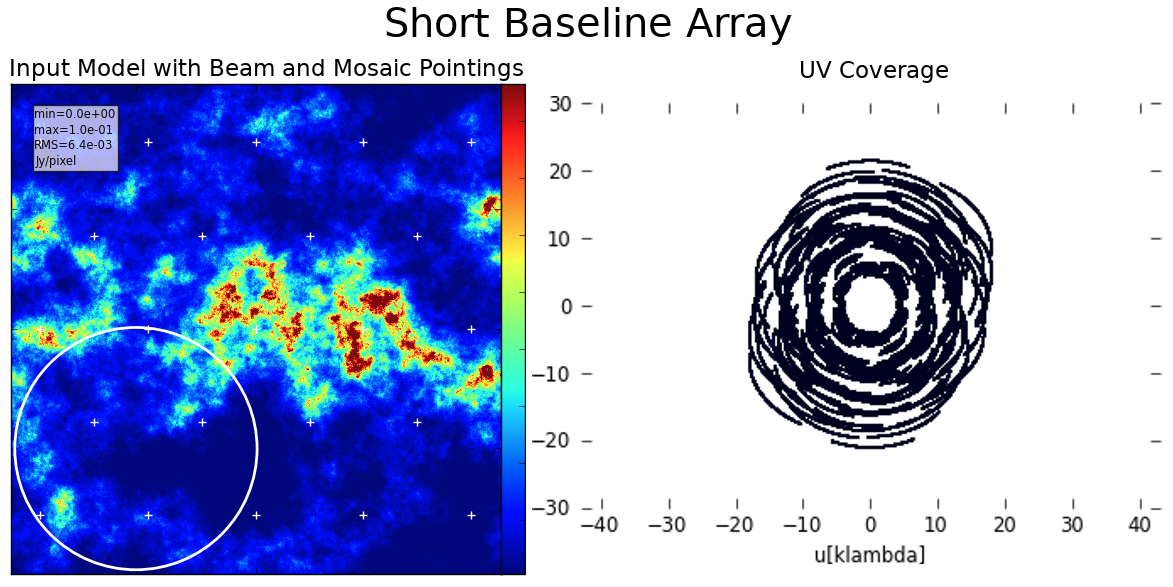
\includegraphics[width=0.8\columnwidth]{figs54/sba.png}
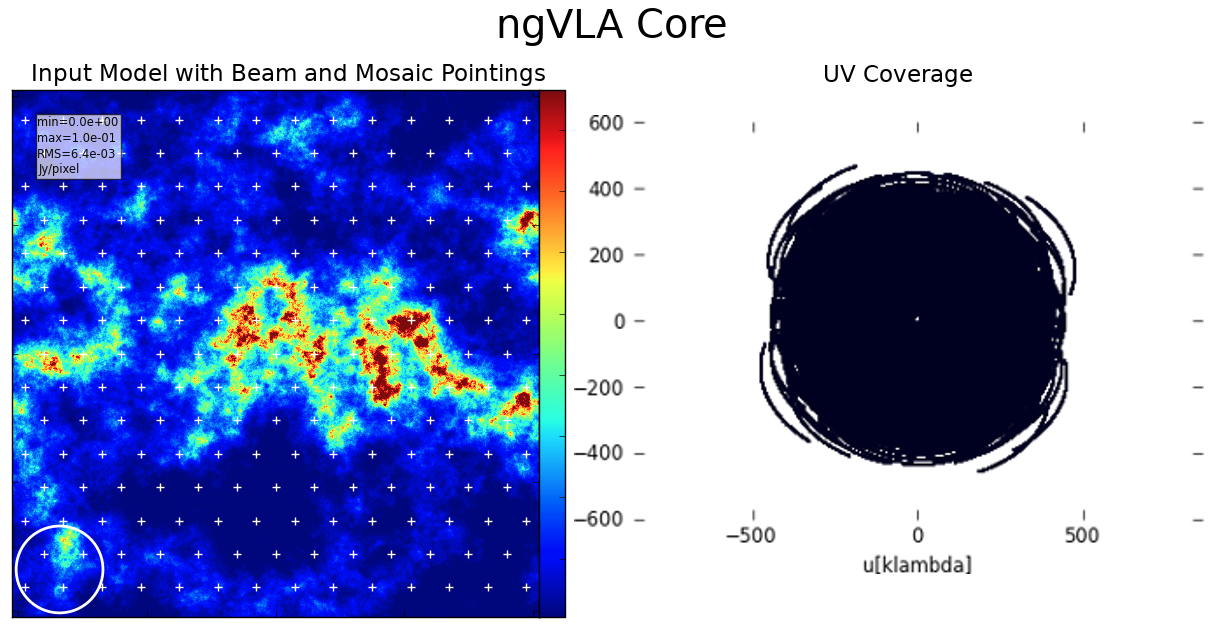
\includegraphics[width=0.8\columnwidth]{figs54/core.png}
\caption{Input model with beam and mosaic pointings overlaid and the UV coverage for the Short Baseline Array (top) and the Core array (bottom). The field-of-view is $\sim$$3^\prime \times 3^\prime$. }
\label{fig:simobserve}

\end{figure}


\begin{figure}
\centering
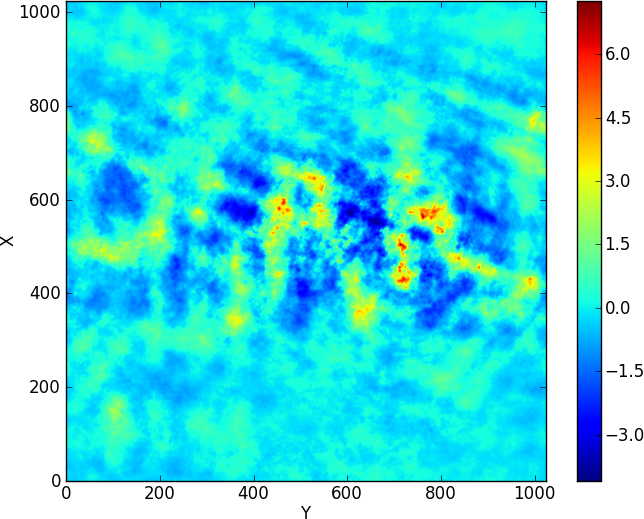
\includegraphics[width=0.4\columnwidth]{figs54/dirty.png} 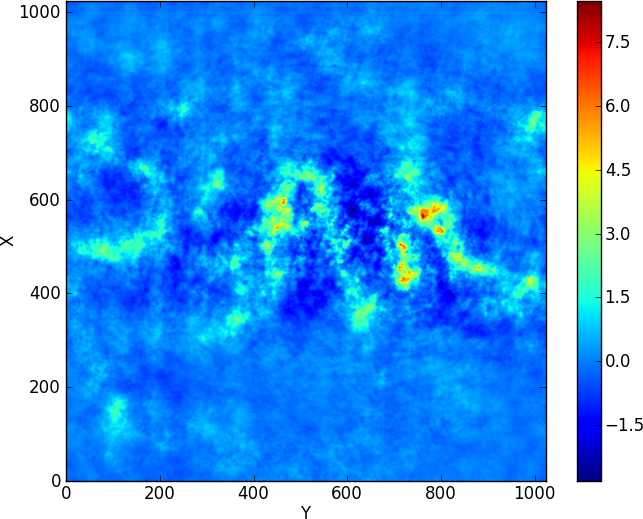
\includegraphics[width=0.4\columnwidth]{figs54/clean.png}
\caption{Primary beam corrected image observing with the SBA and the Core before cleaning (left) and after 8000 iterations of TCLEAN (right). The field-of-view is $\sim$$3^\prime \times 3^\prime$.}
\label{fig:clean}
\end{figure}

\begin{figure}
\centering
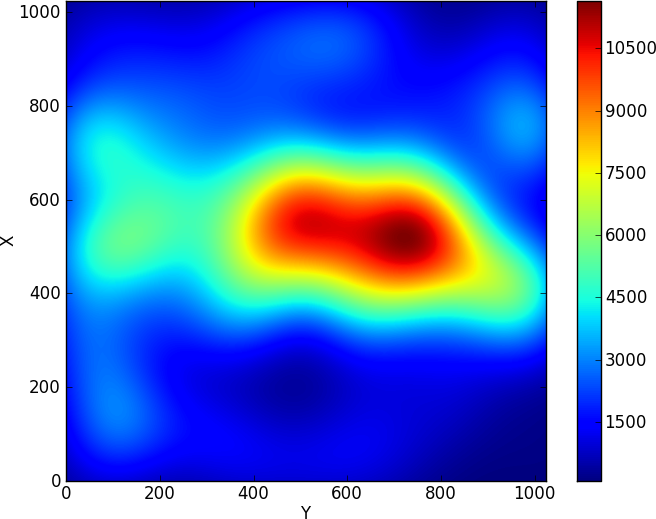
\includegraphics[width=0.325\columnwidth]{figs54/otf18.png} 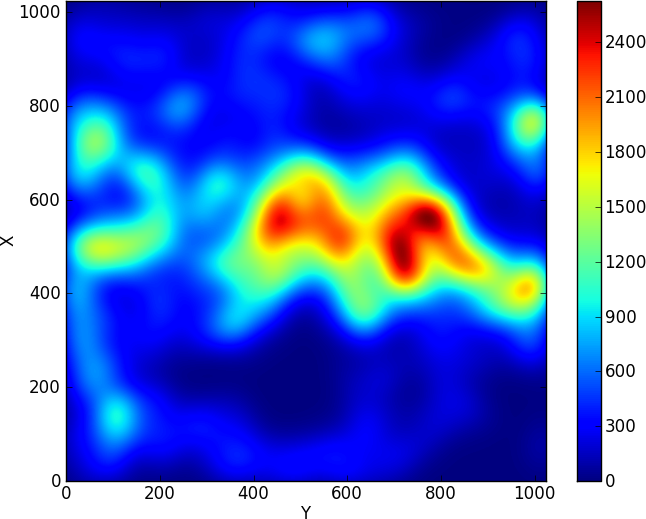
\includegraphics[width=0.325\columnwidth]{figs54/otf45.png} 
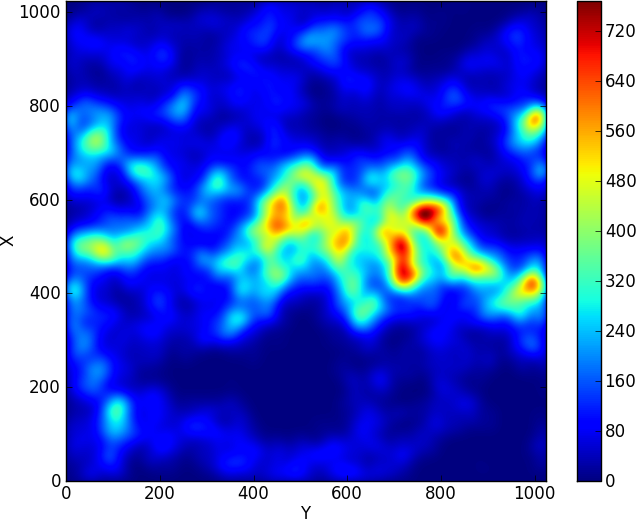
\includegraphics[width=0.325\columnwidth]{figs54/otf100.png}
\caption{`On-the-fly' total power observations from an \SI{18}{\meter} dish (left), a \SI{45}{\meter} dish (middle), and a \SI{100}{\meter} dish (right). The field-of-view is $\sim$$3^\prime \times 3^\prime$.} 
\label{fig:otf}

\end{figure}

\begin{figure}
\centering
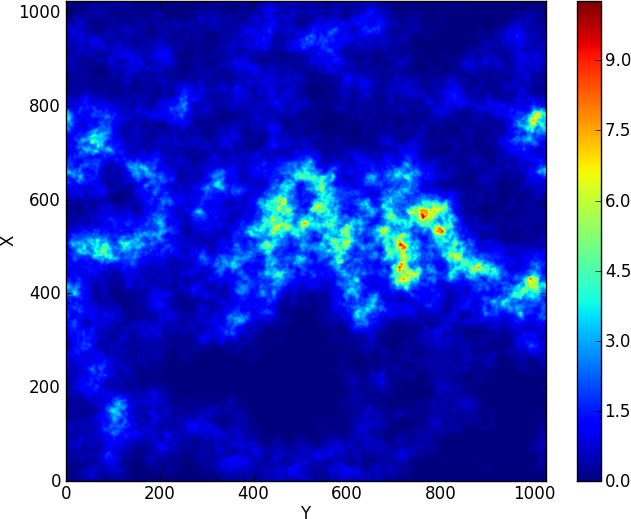
\includegraphics[width=0.4\columnwidth]{figs54/smooth.png} 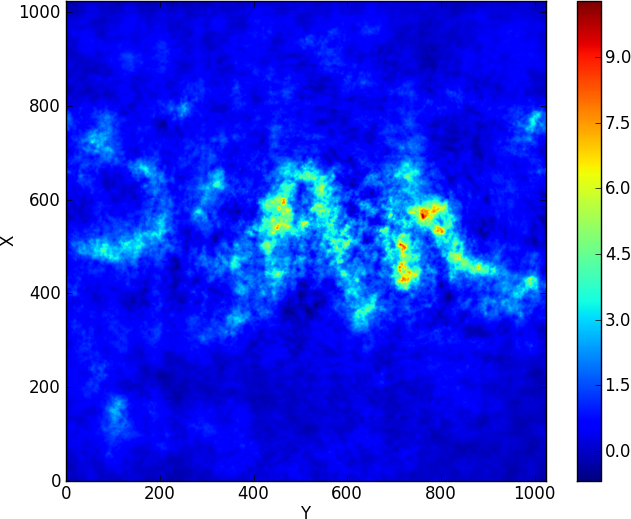
\includegraphics[width=0.4\columnwidth]{figs54/feather18.png}
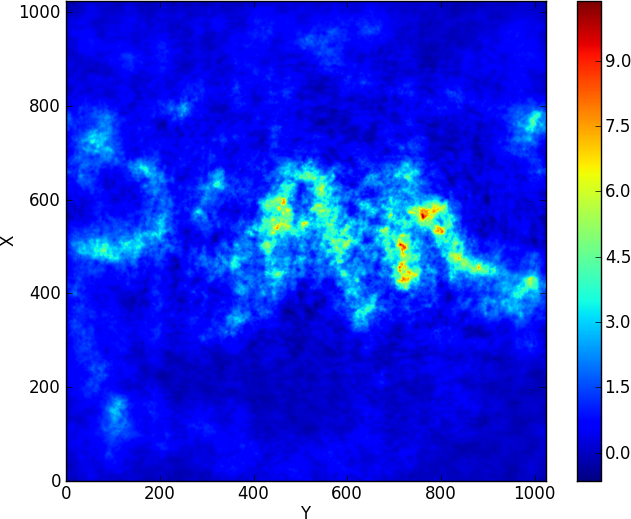
\includegraphics[width=0.4\columnwidth]{figs54/feather45.png} 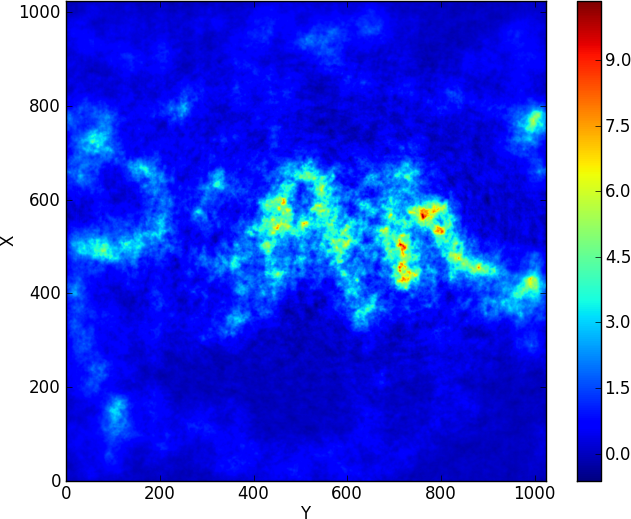
\includegraphics[width=0.4\columnwidth]{figs54/feather100.png}
\caption{The image of input model smoothed to the interferometer beam size (top left) which allows for direct comparison to the feathered images. Primary beam corrected images feathering the interferometric data with the total power from the \SI{18}{\meter} dish (top right), the \SI{45}{\meter} dish (bottom left), and the \SI{100}{\meter} dish (bottom right). The field-of-view is $\sim$$3^\prime \times 3^\prime$.}
\label{fig:feather}

\end{figure}



\begin{table}
\centering
\caption{}
\label{tab:flux}
\def\arraystretch{1.25}
\begin{tabular}{@{} lp{15ex}p{15ex}l @{}}\toprule\midrule
\textbf{Image} 						& \textbf{Total Flux\newline (Jy/beam)} & \textbf{Input Model\newline Difference} & \textbf{Flux Recovery} \\\midrule
Smoothed Input Model 				& 1.12972\e{5} 					& N/A 						& N/A    \\\midrule
Cleaned INT (Core) Map 				& 2.79307\e{3}					& 1.10179\e{5} 				& 2.5\%   \\\midrule
Dirty INT (SBA+Core) Map 			& 1.40705 						& 1.12971\e{5}				& 0\%     \\\midrule
Cleaned INT (SBA+Core) Map			& 9.96528\e{3} 					& 1.03007\e{5}				& 8.82\%  \\\midrule
\SI{18}{\meter} TP + INT Feather	& 1.04002\e{5}					& 8.97000\e{3}				& 92.06\% \\\midrule
\SI{45}{\meter} TP + INT Feather	& 1.09556\e{5}					& 3.41600\e{3}				& 96.98\% \\\midrule
\SI{100}{\meter} TP + INT Feather 	& 1.11600\e{5}					& 1.37200\e{3}				& 98.79\% \\\bottomrule
\end{tabular}
\end{table}

\begin{figure}
\centering
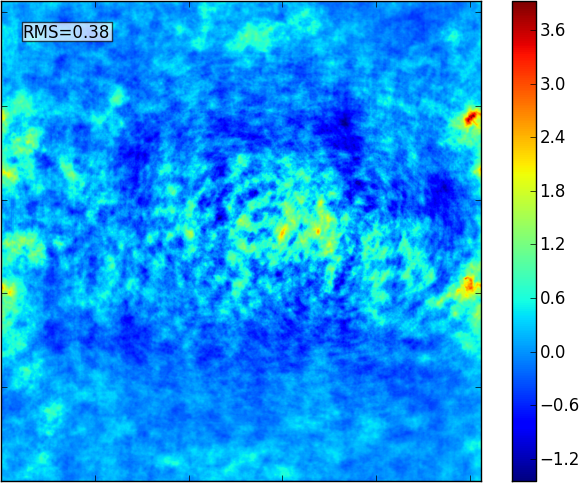
\includegraphics[width=0.325\columnwidth]{figs54/feather18_diff.png} 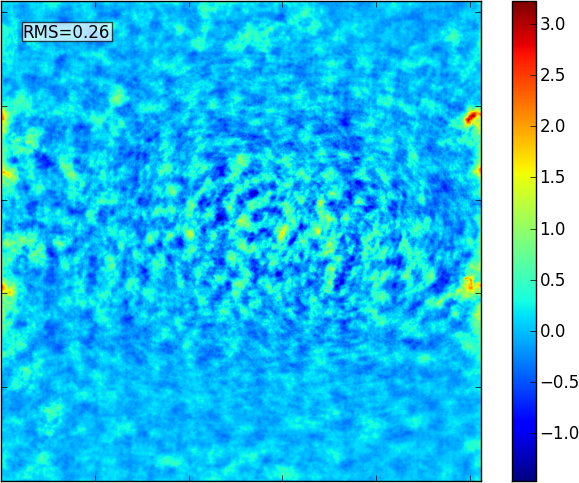
\includegraphics[width=0.325\columnwidth]{figs54/feather45_diff.png}
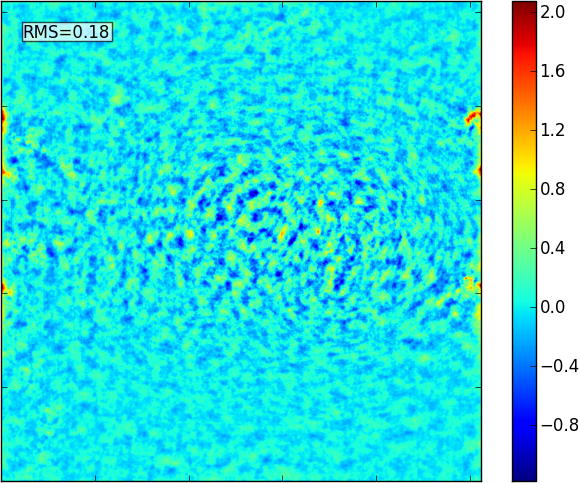
\includegraphics[width=0.325\columnwidth]{figs54/feather100_diff.png}
\caption{Difference maps between the smoothed input model and the \SI{18}{\meter} feathered image (left), the \SI{45}{\meter} feathered image (middle), and the \SI{100}{\meter} feathered image (right). The rms is given in the top left corner of each map. The field-of-view is $\sim$$3^\prime \times 3^\prime$.}
\label{fig:diff}
\end{figure}

\begin{figure}
\centering
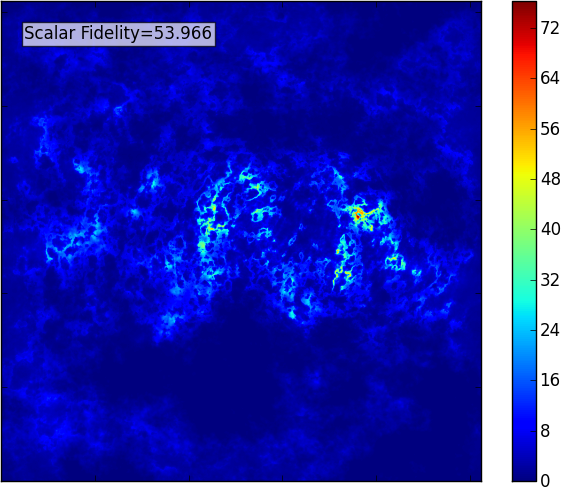
\includegraphics[width=0.325\columnwidth]{figs54/feather18_fidelity.png} 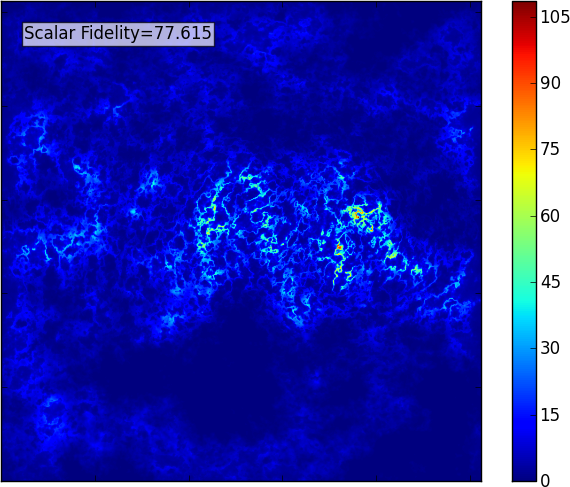
\includegraphics[width=0.325\columnwidth]{figs54/feather45_fidelity.png}
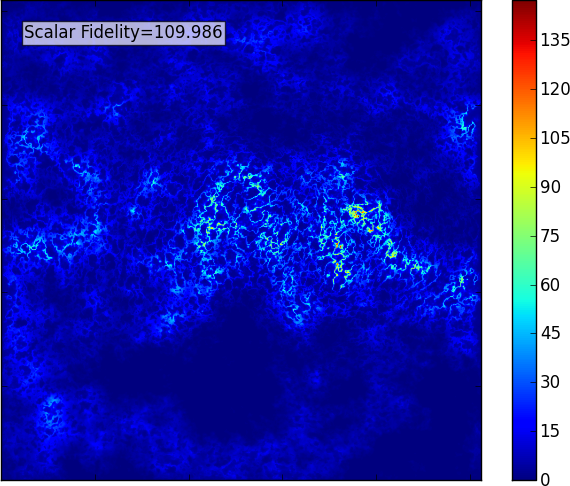
\includegraphics[width=0.325\columnwidth]{figs54/feather100_fidelity.png}
\caption{Fidelity maps for the \SI{18}{\meter} feathered image (left), the \SI{45}{\meter} feathered image (middle), and the \SI{100}{\meter} feathered image (right). The scalar fidelity is given in the top left corner of each map. The field-of-view is $\sim$$3^\prime \times 3^\prime$.}
\label{fig:fid}
\end{figure}


\begin{figure}
\centering
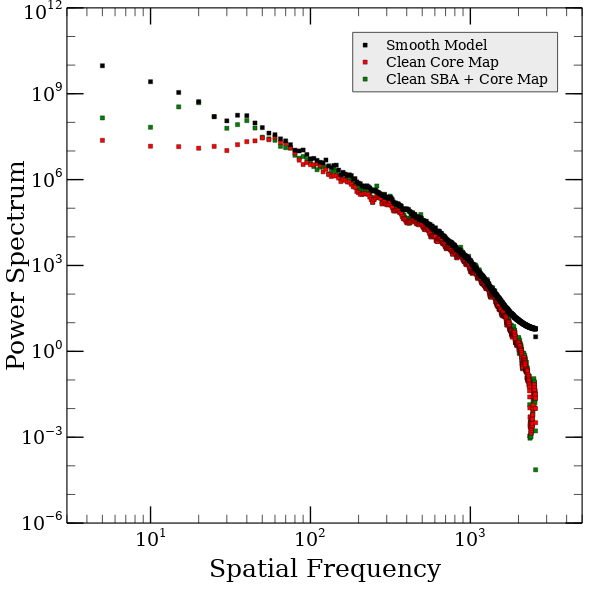
\includegraphics[width=0.49\columnwidth]{figs54/psd1_revised.png}
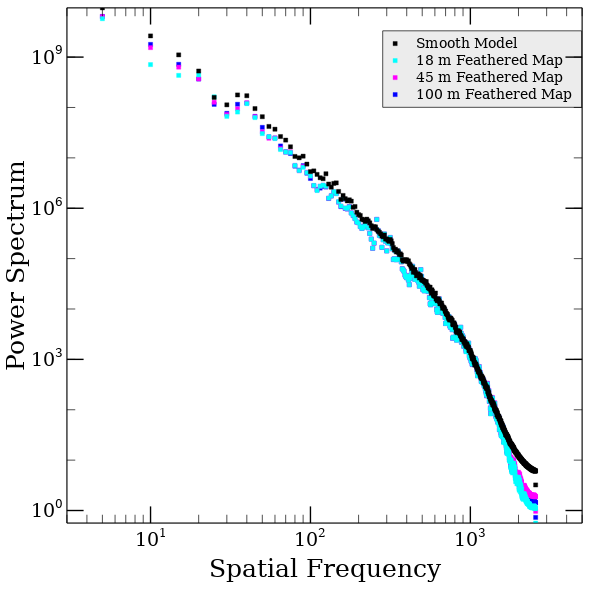
\includegraphics[width=0.49\columnwidth]{figs54/psd2_revised.png}
\caption{Power spectrum density as compared to the smoothed input model (black squares). The left figure shows the power spectrum for the cleaned image with just the ngVLA Core (red) and the cleaned image with both the short baseline array and the core (green). The right figure shows the total power and interferometric feathered images for each single-dish tested: \SI{18}{\meter} dish (cyan), \SI{45}{\meter} dish (magenta), and \SI{100}{\meter} dish (blue).}
\label{fig:psd}
\end{figure}


\end{document}
